\chapter{Selection}
\label{Selection}

This chapter will cover the package selection and the setup of all nodes in the concept. It will also give attention to the configuration of the individual nodes.


The selection process will mainly focus on the defined requirements.

\section{Simulation}
There are many options, when it comes to robot simulation, which makes a selection mandatory. The chosen Simulator then needs to be configured and equipped with models, sensors and a drive system.

\subsection{Selection}
To begin of the selection process a group of reasonable simulators needs to be collected. The two selected options are Gazebo and V-REP since they are the two most used robotics 3D simulators \cite{SimComp}.\\

Both simulators seem to full fill most of the defined requirements to a certain extend, while Gazebo seems to have a easier installation process and integration into ROS since it is included in the default packages of ROS noetic \cite{ROSPkg} since it developed by the Open Source Robotics Foundation as the default simulator for ROS.

As well as Gazebo V-REP offers plugins and URDF conversion for custom models but an even bigger selection of mobile robot models. Which unfortunately can only be used as examples since the required models are very specific.\\
In contrast to V-REP, Gazebo does not contain an integrated model editor.

Based on computational load compared in the Paper of L. Pitonakova et al\cite{Pitonakova} and the setup differences between both simulators, gazebo will be chosen for this project. But both simulators would have been an excellent choice.

\subsection{Model}
Since Gazebo doesn't have an integrated model editor the freeware blender will be used for the model generation of the environment.

As described in the requirements the robot models will be generated using URDF which will be covered later.

\section{Navigation}

As described in the Concept part the ros navigation stack will be used in this project.
The selection of all of its parts will be discussed in the following sections

\subsection{Planners}
Since the planners will consist of two parts (the global planner and the local planner) the nodes of these have to be selected individually.

\subsubsection{global planner}
For the global planner the following two options provided in the navigation stack will be considered 

\begin{itemize}
	\item base\_global\_planner
	\item navfn
\end{itemize}


Here the choice is fairly easy, since base\_global\_planner is the successor of navfn. It still supports the the behavior of navfn, but it offers more options, such as A* planning algorithm instead of Dijkstra.

\todo{A* and Dijkstra explenation in theoretical}


\subsubsection{local planner}
In contrast to the global planner there are way more options for the local planner node. Like the global planners the local planners will be selected using the options offered in the description of the nav\_core.

\begin{itemize}
	\item base\_local\_planner
	\item dwa\_local\_planner
	\item eband\_local\_planner
	\item teb\_local\_planner
	\item mpc\_local\_planner
\end{itemize}\cite{navcore}

To choose the local planner the requirements have to be defined first.
Since the global planner is taking care of the obstacles and the roadlanes the local planner has the general task of following the global path and creating a command velocity that is feasible in regards to the kinematics of the robot.\\

Smooth lane changes are highly wanted in this project. this will help the camera and therefore the road detection to keep seeing the road during swapping the lanes.\\

A time constraint could be used to prevent oscillations around the global path while trying to follow it as close as possible.

As described in its documentation teb\_local\_planner optimizes the trajectory with respect to trajectory execution time, separation from obstacles and compliance with kinodynamic constraints in the runtime.
\todo{cite }





\subsection{costmap}
For the costmap the highly configurable costmap\_2d package will be used. This package is the default package of the navigation\_stack and has no competing packages.
\subsubsection{global costmap}
\subsubsection{local costmap}

\subsubsection{dynamic\_cost\_layer}
Enhancing to the plugins provided in the navigation stack this layer handles inflation of cells with a configurable cost decay and radius.\\

This behaviour can be used to inflate the left road marking in the global costmap to force the global plan on the right side of the road. The plugin can also be used to inflate cells with zero cost, which is useful to guarantee a free right lane or to give some free space around obstacles located on the road.\\

The layer receives a message of type sensor\_msgs::PointCloud on a configurable topic. This PointCloud is expected to feature Channel Values for the inflation radius, the maximal and the minimal cost for each individual point.\\

Since we can't assume that the incoming points will be in the frame of the costmap the points in the costmap have to be transformed into the right frame using tf2.\\

To minimize the computation load a bresenham based algorithm for the circle rasterization will be used. Now the point symmetry around the cell can be used to further minimize the computational load and only $\frac{1}{8}$th of the circle has to be computed. The rasterization process can be described by the following image.\\

Adding to the typical behavior of the bresenham rasterization the area of the circle will be filled with the cost specified for the point. For this a linear decaying \nth{1} degree function will be used which requires the computation of the distance of the cell to the center of the circle.\\ Since this will still require the usage of a square root for each cell in the circle This will be optimized as well.\\

The goal here is to use a function that contains only the squared distance, which still represents a decaying trend. This requirement rules out every function with an odd degree, as well as all functions with an x offset. This leaves all functions with an even degree from which we choose the \nth{2} degree function to reduce square operators. The comparison between the two functions can be seen in the picture below.

\center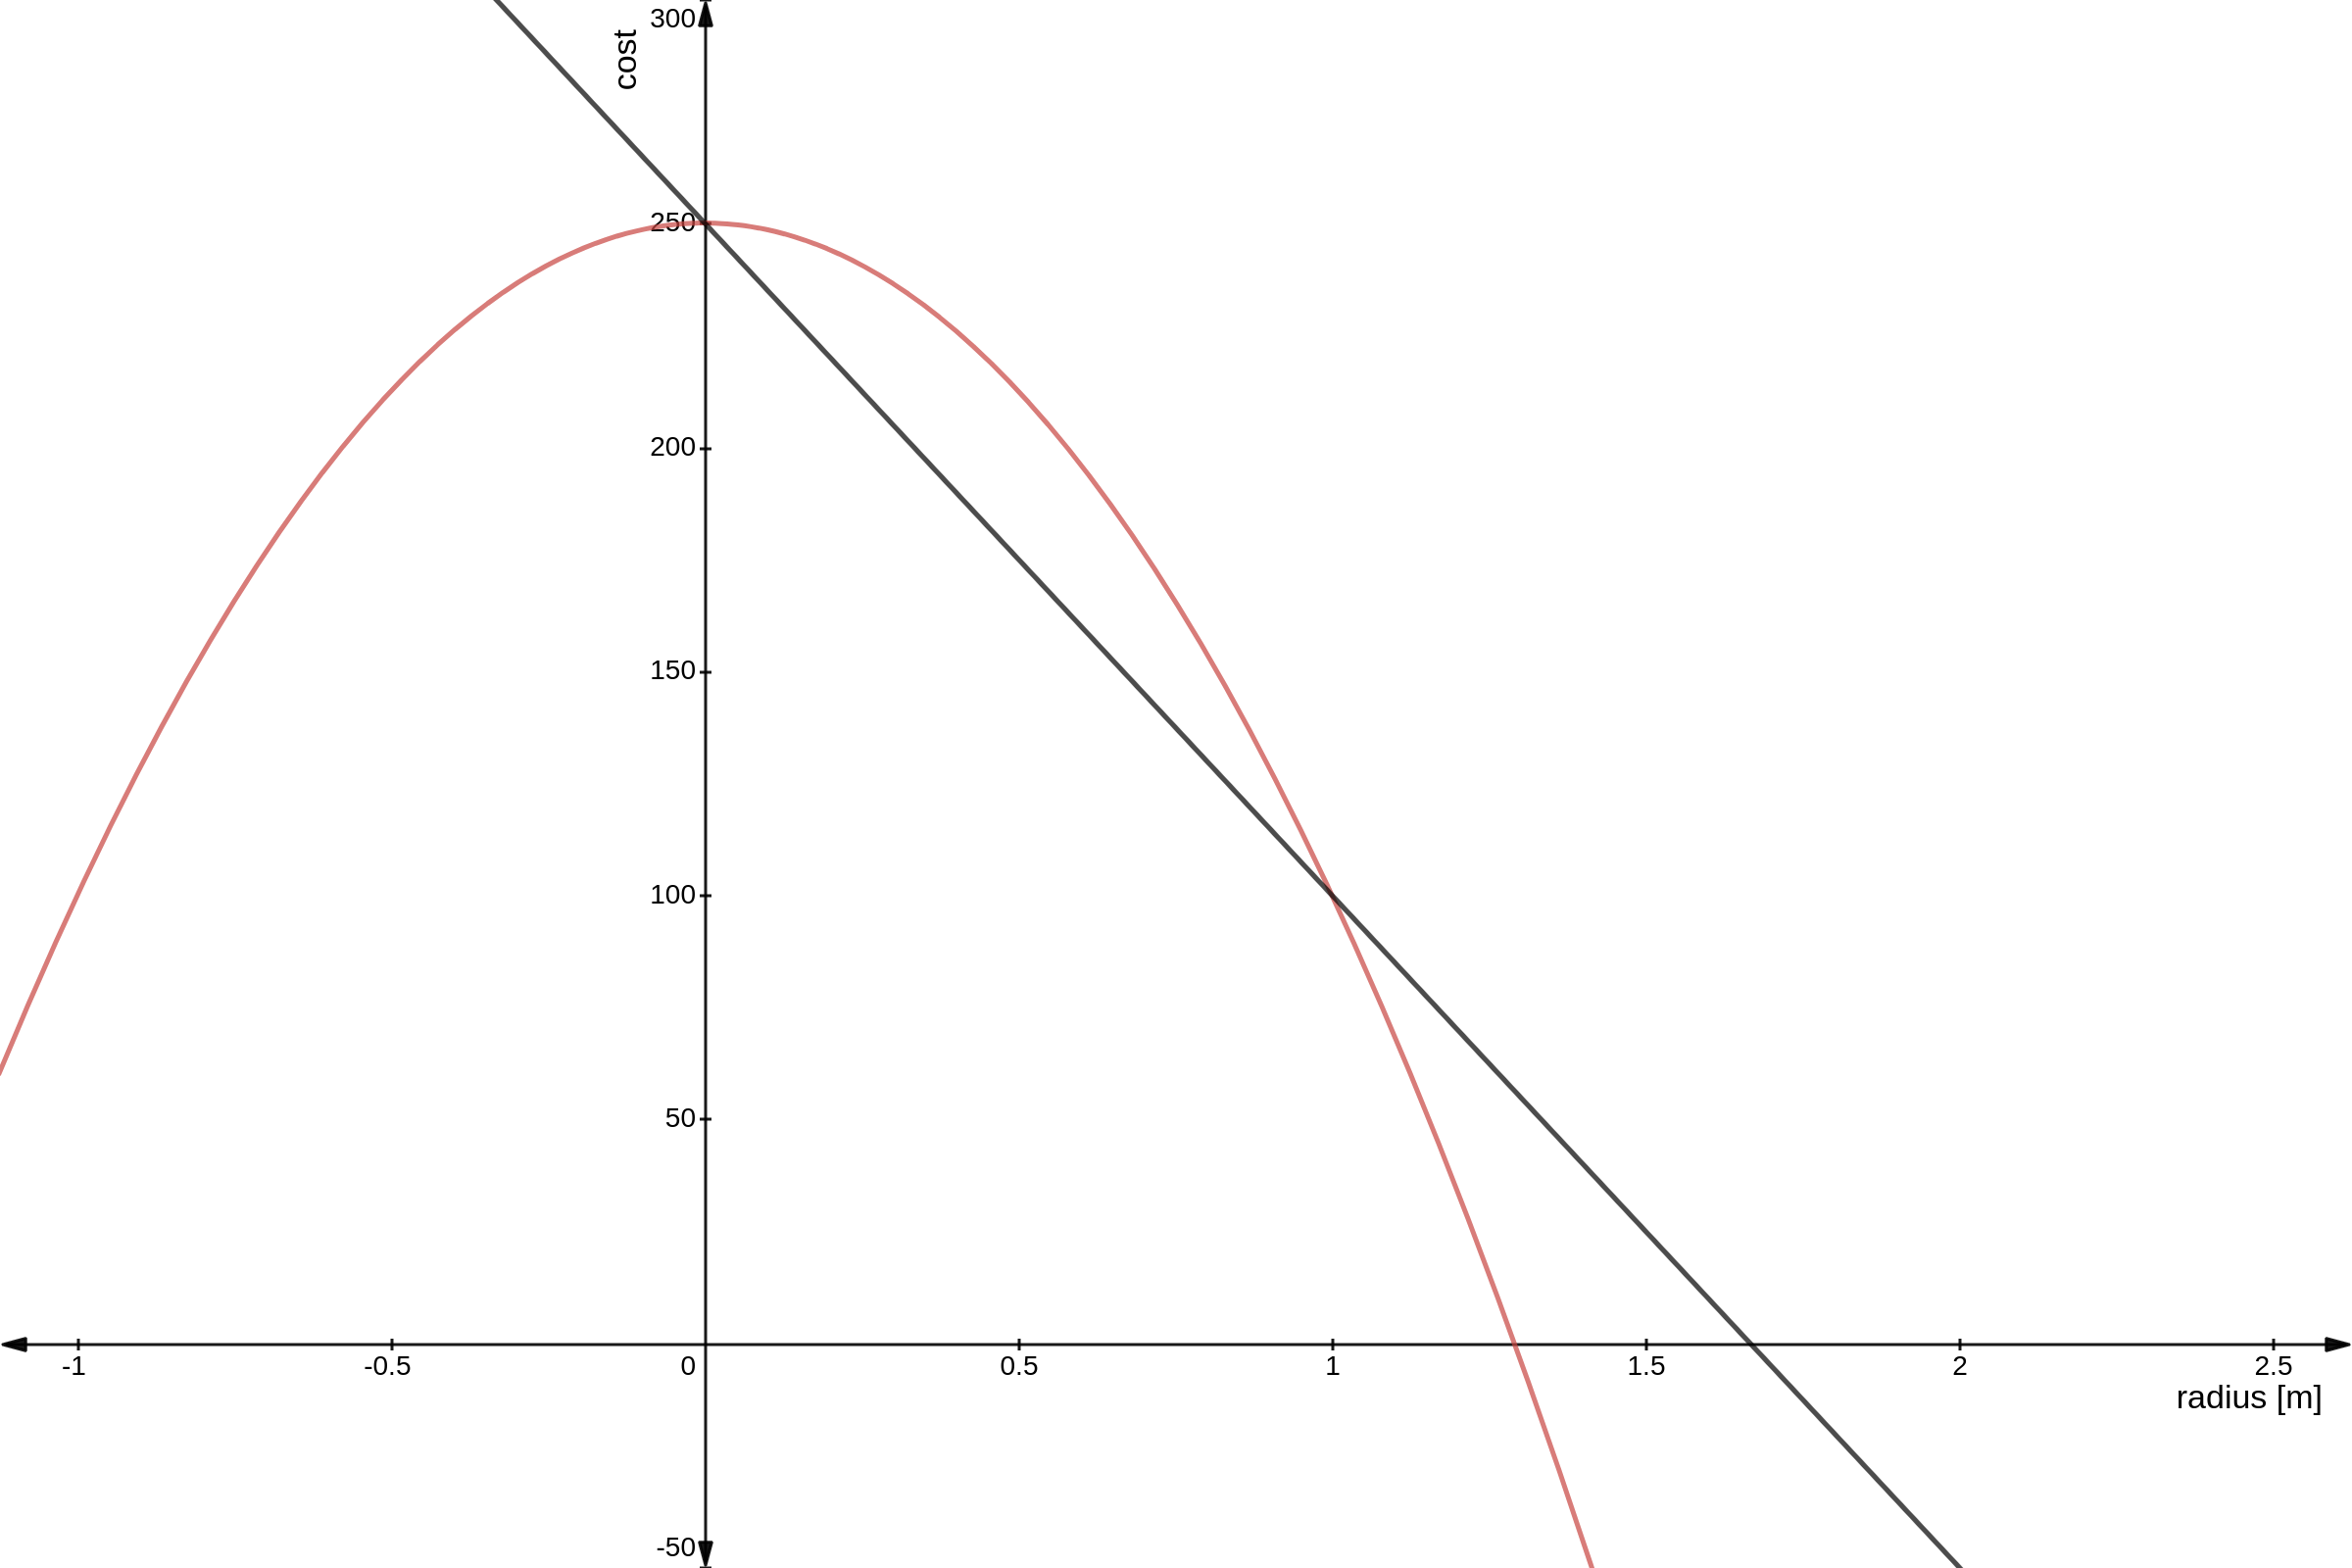
\includegraphics[width=140mm]{Pictures/linear cost comparison}



\section{Odometry}

\subsection{Encoder}
\subsection{IMU}
\subsection{Improvement using SLAM}

\section{Laser\_Filter}

\section{PoseFinder}
This Node is part of the arlo\_navigation package. Its job is, to find the pose of the next possible goal and send it to the move\_base action client.
Based on the data we gather from the observing sensors the only two sources to gather data about the road situation in front of the robot is the extracted camera data and the data from the last time the robot was in the same area than can be found in the map generated by SLAM.
Since we don't have the map in the first round of the robot gathering goals from the live camera data is more important. 
\subsection{Using current camera data}
The easiest way to get new goals would be to take the last point of the polynomial provided by the road detection as the position and calculate the yaw angle of the new goal with the gradient of the last two.\\

While this is a logical approach in an ideal scenario, it certainly will not work in a realistic one since we can't assure a continuous data stream from the road detection.\\

This is mostly caused by the camera not always seeing enough of the road which can for example be caused by the following reasons:

\begin{itemize}
	\item obstacle covering the markings
	\item while driving a corner the camera isn't always pointed tangential to the curvature
	\item steering during obstacle avoidance
	\item noise in camera data
\end{itemize}


This suggest that a prediction for the possible upcoming road is needed. To a small extend this is provided by the polynomials of the road detection, but the have a restricted domain, after which the error will rapidly increase.

\subsection{Approximations}

Since the road mostly consists of circles of varying radii and origins, it is self evident, that using the polynomials in their restricted domain to represent a section of a circle will give a better estimate.\\
This circle can be calculated using the following linear least-square approach:\\

In theory this approximation should work for almost straight sections as well, but the radius and the origin will trend to infinity and caused by the camera noise and the inaccuracy of the road detection the representation of the road will get worse and worse.\\

This leads to the following linear least square approach for straight lines:\\

Switching between the result of the two approximations will result in the best result for both scenarios. This switching will be triggered by the radii of the approximated circles exceeding a configurable threshold.\\

The next step is a goal extraction from the chosen approximation. This goal will be calculated at a given distance from the robot origin on the approximated route. In contrast to the approximated lines, the circles have a defined angle of trustworthiness. Otherwise small circles would cause the goal to be way of the prediction. The orientation of the goal will then be determined using the differentiation of the function.\\

With the calculated points on either both circles or on both lines the mean can be calculated and represents the new goal for the robot.



\subsection{goal from map}

If the robot is running a SLAM algorithm during the first round the map should be finished once the robot passes its start point. Then the approximation is unnecessary since extracting goals directly from the slam map is more efficient and provides goals that will  always be on the road. Furthermore the distance, at which goals will be found can be increased, which results in higher speeds and/or lower planner frequencies.\\

To find a goal in the SLAM map a circle rasterization algorithm will be used.\\

This algorithm finds every cell on a circular path around the robot and its associated value in the map. The values outside of a given FOV (field of view) can be eliminated. Then the remaining values with a larger likelihood than a configurable threshold will be reduced to one point by taking the mean value of all of them.\\

The orientation of the goal is then determined by using the approximation algorithms.


\section{MarkFreeSpace}

The purpose of this node is to provide data to the SLAM algorithm as well as to the costmaps. This data consists from the points on the polynomials of the road detection in combination with the filtered points of the laser scan.\\

For SLAM and the obstacle layer of the costmap the node simply transforms the data into the same frame and casts it into the form of a sensor\_msgs::PointCloud2.\\

The data of the dynamic cost layer has to contain more information. It is in the form of a sensor\_msgs::PointCloud and contains channel values for point individual inflation radius, min-cost and max-cost. By giving the Layer point individual inflation parameters the node provides information about the cells on the left road marking that need to have inflated cost values and information about the points on the right road marking that should have a clean zone around them. Furthermore the node provides points of obstacles that are on the road and clears the inflated cost around it. Which will allow the global planner to make a plan for passing the obstacle.

\section{SLAM}





